\documentclass[reprint, nofootinbib, 10pt]{revtex4-2}

\usepackage[T2A]{fontenc}			% кодировка
\usepackage[utf8]{inputenc}			% кодировка исходного текста
\usepackage[english,russian]{babel}	% локализация и переносы

\usepackage{amsmath,amsfonts,amssymb,amsthm,mathtools}

\usepackage[usenames]{color}
\usepackage{colortbl}
\usepackage{indentfirst} %Красная строка
\usepackage{hyperref}

\usepackage{booktabs}
\usepackage{graphicx}  % Для вставки рисунков
\graphicspath{{images/}{graphs/}}  % папки с картинками

\renewcommand*{\thefootnote}{\alph{footnote}}

\begin{document}

\title{Изучение спектров атома водорода и молекулы йода}
\author{Илларионов Владислав}
\affiliation{группа Б04-855}

\maketitle



\section*{Введение}


В ходе данной работы исследуются спектральные закономерности в оптических спектрах атома
водорода и молекулы йода. По результатам измерений вычисляется постоянная Ридберга для
водорода и энергии диссоциации для молекулы йода в основном, а также в возбужденном состоянии.


\section*{Теоретическая часть}


\subsection*{Изучение спектра атома водорода}

Длины волн спектральных линий водородоподобного атома описываются \textit{обобщенной формулой Бальмера}:

\begin{equation}
	\label{eq:balmer}
	\frac{1}{\lambda_{mn}} = R Z^2 \left( \frac{1}{n^2} - \frac{1}{m^2} \right),
\end{equation}

где $R$~--- константа, называемая \textit{постоянной Ридберга}, $Z$~--- атомный номер,
а $m$ и $n$~--- целые числа.

В данной работе изучается \textit{серия Бальмера}, линии которой лежат в видимой области. Для серии
Бальмера $n=2$, а величина $m$ для первых четырех линий принимает значения 3, 4, 5, 6 соответственно.
Эти линии обозначаются символами $H_\alpha$, $H_\beta$, $H_\gamma$, $H_\delta$.


\subsection*{Изучение молекулярного спектра йода}

Молекулы обладают более богатым спектром возбужденных состояний, чем изолированные атомы.
В то время как возбуждения атомов это переходы их электронов на более высоко расположенные
энергетические уровни, в молекулах могут возбуждаться дополнительные степени свободы.
В первом приближении энергия молекулы может быть представлена в виде:

\begin{equation}
	E = E_{\text{эл}} + E_{\text{колеб}} + E_{\text{вращ}}
\end{equation}

Однако характерная энергия вращательных движений в $10^6$ раз меньше энергии электронных переходов,
и поэтому наблюдение вращательных переходов оптическими спектрометрами невозможно.
На рис.~\ref{fig:enrglvls} схематически изображены энергетические уровни молекулы без учета вращательной
структуры. Штриховыми линиями показаны чисто электронные уровни $E_1$ и $E_2$, а сплошными колебательные
подуровни этих состояний.

\begin{figure}[ht]
	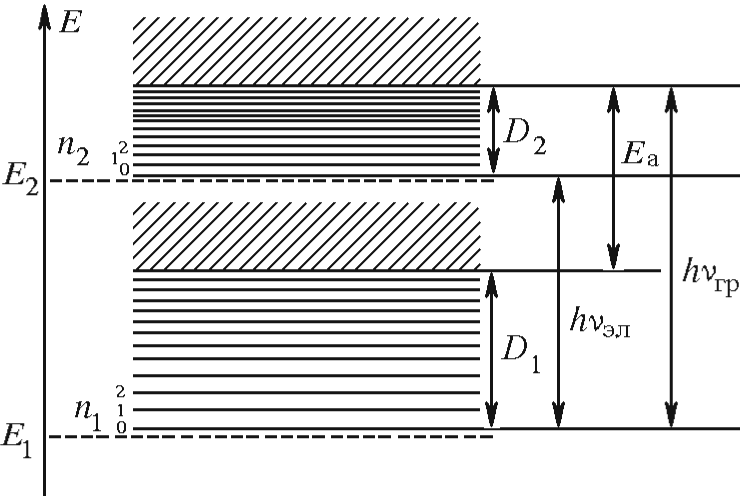
\includegraphics[width=\linewidth]{energy_levels.png}
	\caption{Электронные и электро-колебательные уровни двухатомной молекулы}
	\label{fig:enrglvls}
\end{figure}

Энергетическое положение линий поглощения описывается выражением:

\begin{equation}
	\label{eq:molecule_energy}
	h \nu_{0, n_2} = (E_2 - E_1) + h \nu_2 \left( n_2 + \frac{1}{2} \right) - \frac{h \nu_1}{2}
\end{equation}


\section*{Экспериментальная установка}

Для измерения длин волн спектральных линий в работе используется стеклянно-призменный
монохроматор-спектрометр УМ-2.

Основные элементы монохроматора представлены на рис. \ref{fig:spectrometer}.

\begin{enumerate}
	\item Входная щель 1, снабженная микрометрическим винтом 9.
	\item Коллиматорный объектив 2, снабженный микрометрическим винтом 8.
	\item Сложная спектральная призма 3, состоящая из трех склеенных призм П$_1$, П$_2$, П$_3$,
		и установленная на поворотном столике 6.
	\item Поворотный столик 6, вращающийся вокруг вертикальной оси при помощи микрометрического
		винта 7 с отсчётным барабаном. На барабан нанесена винтовая дорожка с градусными делениями.
		Вдоль дорожки скользит указатель барабана.
	\item Зрительная труба, состоящая из объектива 4, окуляра 5 и указателя 10.
	\item Массивный корпус 11, предохраняющий прибор от повреждений и загрязнений.
	\item Оптическая скамья, на которой могут перемещаться рейтеры с источником света Л и
		конденсором К.
\end{enumerate}

\begin{figure}[ht]
	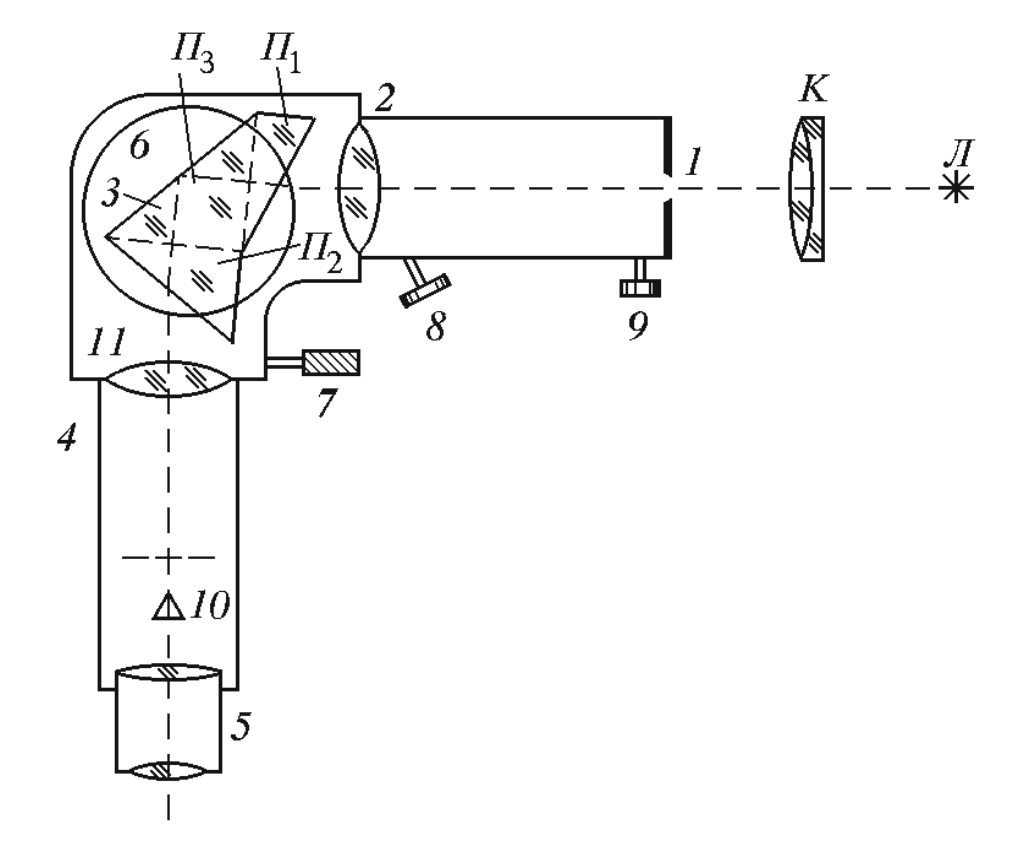
\includegraphics[width=0.7\linewidth]{spectrometr.png}
	\caption{Устройство монохроматора УМ-2}
	\label{fig:spectrometer}
\end{figure}

\section*{Методика измерения}

Спектрометр нуждается в предварительной градуировке по известным спектральным линиям ртути и
неона. Ртутная лампа применяется для градуировки в коротковолновой части спектра,
а неоновая~--- в длинноволновой и средней.

Далее по градуировочной кривой определяются длины волн линий $H_\alpha$, $H_\beta$, $H_\gamma$,
$H_\delta$, а также линий поглощения йода $n_{1, 0}$ (одна из самых длинноволновых хорошо видимых линий поглощения),
$n_{1, 5}$ (шестая по счёту от выбранной длинноволновой линии) и $n_{\text{гр}}$ (граница схождения спектра).
Энергии соответствующие этим линиям обозначим как $h \nu_{1, 0}$, $h \nu_{1, 5}$ и $h \nu_{\text{гр}}$ соответственно.

Основную ошибку в вычисления вносит погрешность аппроксимации. Она будет оценена как стандартное отклонение
истинных значений длин волн спектральных линий неона и ртути и значений, полученных с помощью аппроксимирующего
полинома.

\section*{Обработка данных}


\subsection*{Спектр водорода}

Аппроксимируя экспериментальные данные (табл.~\ref{tab:hg_calibrating}-\ref{tab:neon_calibrating})
полиномом 5-ой степени, построим градуировочную кривую (см.~рис.~\ref{graph:calibrating}).
Аппроксимирующий многочлен имеет следующий вид:

\begin{eqnarray*}
	f(x) = 3.6 \cdot 10^{-14} x^5 - 2.4 &&\cdot 10^{-10} x^4 + 7 \cdot 10^{-7} x^3 -\\
	&&- 8.9 \cdot 10^{-4} + x + 3593
\end{eqnarray*}

Далее рассчитаем длины волн спектральных линий водорода и йода.
Для каждой из спектральных линий водорода с помощью формулы~(\ref{eq:balmer})
найдем значение постоянной Ридберга~(см.~табл.~\ref{tab:ridbergs}),
и вычислим среднее.

\[ R_{mean} = 109814 \pm 71 \text{ см}^{-1} \]
\[ R_{\text{табл}} = 109678 \text{ см}^{-1} \]

\begin{figure}[ht]
	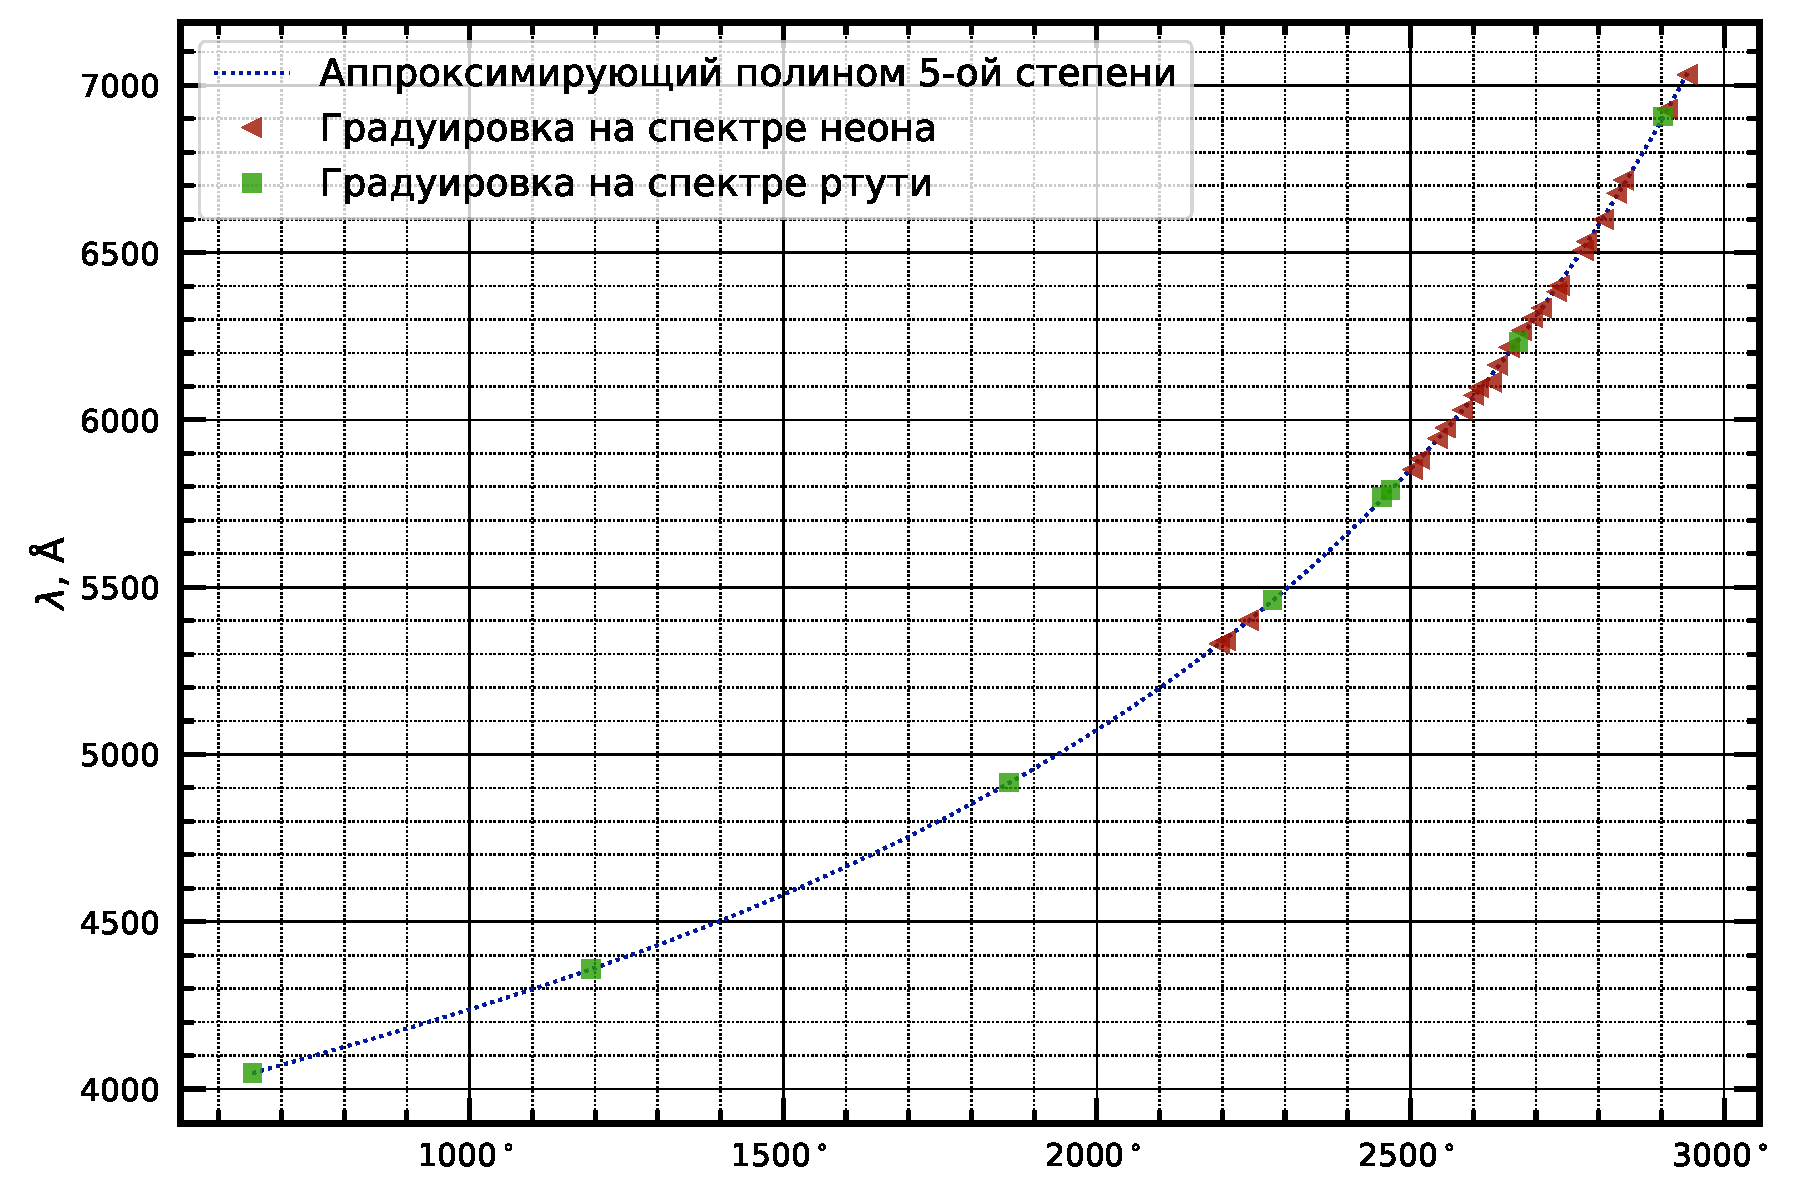
\includegraphics[width=\linewidth]{calibrating.pdf}
	\caption{Градуировка монохроматора}
	\label{graph:calibrating}
\end{figure}


\subsection*{Спектр йода}

Энергия колебательного кванта возбужденного состояния молекулы йода определяется как:
\[ h \nu_2 = (h \nu_{1,5} - h \nu_{1,0})/5 = 0.016 \pm 0.001 \text{эВ} \]

Учитывая, что энергия колебательного кванта основного состояния $h \nu_1 = 0.027$ эВ,
энергия возбуждения атома $E_A = 0.94$ эВ,
с помощью формулы~(\ref{eq:molecule_energy}) рассчитаем энергию электронного перехода
$h \nu_{\text{эл}}$, энергию диссоциации в основном состоянии $D_1$ и в возбужденном~--- $D_2$.

\begin{subequations}
	\begin{equation*}
		h \nu_{\text{эл}} = h \nu_{1, 0} - \frac{3 h \nu_2}{2} + \frac{h \nu_1}{2} = 1.975 \pm 0.003 \text{ эВ}
	\end{equation*}
	\begin{equation*}
		D_1 = h \nu_{\text{гр}} - E_A = 1.51 \pm 0.01 \text{ эВ}
	\end{equation*}
	\begin{equation*}
		D_2 = h \nu_{\text{гр}} - h \nu_{\text{эл}} = 0.477 \pm 0.05 \text{ эВ}
	\end{equation*}
\end{subequations}


\section*{Вывод}

В ходе данной работы методом спектрального анализа были получены значения постоянной Ридберга
для водорода, а также энергии диссоциации молекулы йода.

Табличное значение постоянной Ридберга не попадает в 68\% доверительный интервал значения,
полученного экспериментально. Предположительно это может быть связано с тем, что в диапазон
длин волн спектральных линий водорода попало мало точек градуировки и аппроксимация
не правильно описывает связь длины волны и делений барабана спектрометра.


\newpage
\appendix

\vspace*{1cm}
\section{Таблицы}

\begin{table}[h!]
\centering
\caption{Градуировка на спектре ртути}
\label{tab:hg_calibrating}
\begin{tabular}{lcccr}
\toprule
№ & {\hspace{0.8cm}} & $\lambda$, Å & {\hspace{0.8cm}} & $^\circ$ \\
\midrule
K1 & {} & 6907 & {} & 2902 \\
K2 & {} & 6234 & {} & 2672 \\
1  & {} & 5791 & {} & 2468 \\
2  & {} & 5770 & {} & 2454 \\
3  & {} & 5461 & {} & 2280 \\
4  & {} & 4916 & {} & 1860 \\
5  & {} & 4358 & {} & 1194 \\
6  & {} & 4047 & {} &  654 \\
\bottomrule
\end{tabular}
\end{table}


\begin{table}[h!]
	\centering
	\caption{Градуировка на спектре неона}
	\label{tab:neon_calibrating}
	\begin{minipage}[h]{0.49\linewidth}
		\begin{tabular}{lcccr}
\toprule
№ & {\hspace{0.5cm}} & $\lambda$, Å & {\hspace{0.5cm}} & $^\circ$ \\
\midrule
1  & {} & 7032 & {} & 2942 \\
2  & {} & 6929 & {} & 2910 \\
3  & {} & 6717 & {} & 2840 \\
4  & {} & 6678 & {} & 2830 \\
5  & {} & 6599 & {} & 2808 \\
6  & {} & 6533 & {} & 2782 \\
7  & {} & 6507 & {} & 2776 \\
8  & {} & 6402 & {} & 2738 \\
9  & {} & 6383 & {} & 2734 \\
10 & {} & 6334 & {} & 2710 \\
11 & {} & 6305 & {} & 2696 \\
12 & {} & 6267 & {} & 2678 \\
13 & {} & 6217 & {} & 2658 \\
\bottomrule
\end{tabular}

	\end{minipage}
	\begin{minipage}[h]{0.49\linewidth}
		\begin{tabular}{lcccr}
\toprule
№ & {\hspace{0.5cm}} & $\lambda$, Å & {\hspace{0.5cm}} & $^\circ$ \\
\midrule
14 & {} & 6164 & {} & 2640 \\
15 & {} & 6113 & {} & 2630 \\
16 & {} & 6096 & {} & 2610 \\
17 & {} & 6074 & {} & 2602 \\
18 & {} & 6030 & {} & 2584 \\
19 & {} & 5976 & {} & 2556 \\
20 & {} & 5945 & {} & 2544 \\
21 & {} & 5882 & {} & 2516 \\
22 & {} & 5852 & {} & 2504 \\
23 & {} & 5401 & {} & 2242 \\
24 & {} & 5341 & {} & 2206 \\
25 & {} & 5331 & {} & 2196 \\
{} & {} &   {} & {} &    {} \\
\bottomrule
\end{tabular}

	\end{minipage}
\end{table}

\begin{table}
\centering
\caption{Постоянная Ридберга, рассчитанная для разных спектральных линий водорода}
\label{tab:ridbergs}
\begin{tabular}{lrcccc}
\toprule
{} &    $^\circ$ & {} &  $\lambda$, Å & {} & $R$, см$^{-1}$ \\
\midrule
$H_\alpha$ &  2790 & {} & $6554 \pm 8$ & {} & $109849 \pm 129$ \\
$H_\beta$  &  1800 & {} & $4852 \pm 8$ & {} & $109913 \pm 174$ \\
$H_\gamma$ &  1164 & {} & $4338 \pm 8$ & {} & $109755 \pm 195$ \\
$H_\delta$ &   754 & {} & $4100 \pm 8$ & {} & $109738 \pm 206$ \\
\bottomrule
\end{tabular}
\end{table}





\end{document}